\documentclass[dvipdfmx]{beamer}

\usepackage{bxdpx-beamer}
\usepackage{hyperref}
\usepackage{pxjahyper}
\usepackage{minijs}
\usepackage{lmodern}
\usepackage{xcolor}
\usepackage{amsmath, amssymb, mathtools, bm}

\usepackage{ulem}
\newcommand{\fuee}{:;($\cap \ \acute{}$ \uwave{$\quad \ $} $\grave{} \ \cap$);:}

\newcommand{\pf}[2]{\frac{\partial{#1}}{\partial{#2}}}
\renewcommand{\d}[2]{\delta_{#1}^{#2}}
\newcommand{\g}[2]{g_{#1}^{#2}}
\newcommand{\s}[2]{s_{#1}^{#2}}
\renewcommand{\u}[2]{u_{#1}^{#2}}
\newcommand{\w}[2]{w_{#1}^{#2}}
\newcommand{\x}[2]{x_{#1}^{#2}}
\newcommand{\z}[2]{z_{#1}^{#2}}
\renewcommand{\kanjifamilydefault}{\gtdefault}

\newtheorem{thm}{定理}
\usefonttheme{professionalfonts}
\usetheme{Madrid}
\setbeamertemplate{navigation symbols}{}
\setbeamertemplate{itemize item}[circle]
\setbeamertemplate{itemize subitem}[circle]
\setbeamertemplate{enumerate item}[default]


\title{LSTM}
\author{吉永 塁}
\date{2020年6月17日}


\begin{document}

\begin{frame}[plain,noframenumbering]
    \titlepage
\end{frame}


\begin{frame}
    \frametitle{内容・参考文献}
    内容 : LSTMについて,特にLSTMが教科書\cite{blue}に掲載されている形になるまでの流れを中心に.
    \begin{itemize}
        \item 記号の使い方は\cite{blue}に準じました.
        \item 指摘・補足があればお願いします.
    \end{itemize}

    \vspace{\baselineskip}

    \begin{thebibliography}{9}
        \beamertemplatetextbibitems
        \bibitem{blue}  岡谷貴之. "深層学習" 第7章再帰型ニューラルネット
        \bibitem{ulstm} "わかるLSTM $\sim$ 最近の動向と共に"
        {\footnotesize \url{https://qiita.com/t_Signull/items/21b82be280b46f467d1b}}
        \bibitem{orig} S.Hochreiter and J.Schmidhuber. "LONG SHORT-TERM MEMORY"
    \end{thebibliography}
\end{frame}


\begin{frame}
    \frametitle{LSTM 概要図}
    \begin{figure}
        \centering
        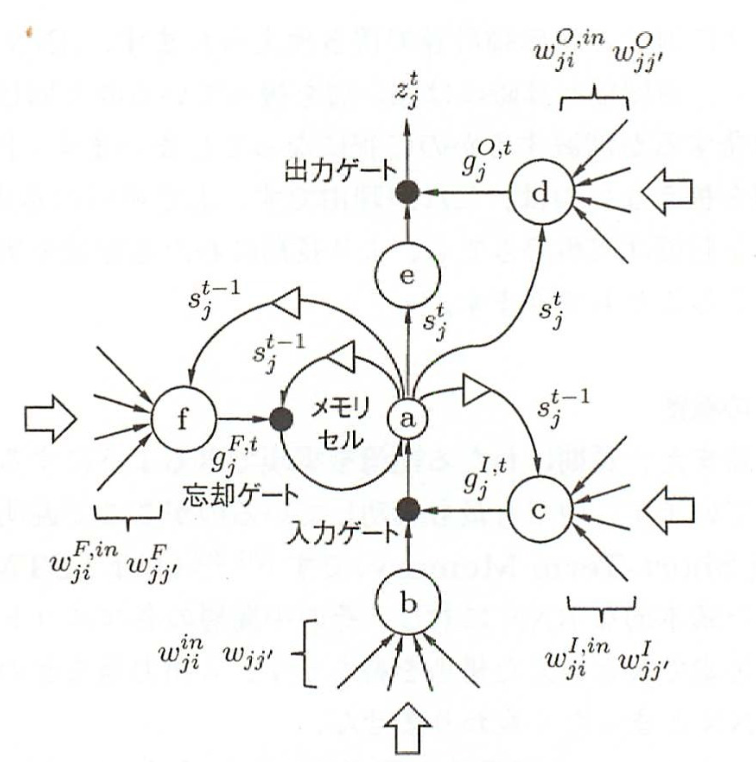
\includegraphics[scale=0.25]{figure/lstm.png}
    \end{figure}
    \flushright{{\small \fuee}}
\end{frame}


\begin{frame}
    \frametitle{Recurrent Neural Network}
    \begin{columns}
        %%% figure - left
        \begin{column}[T]{0.20\textwidth}
            \centering
            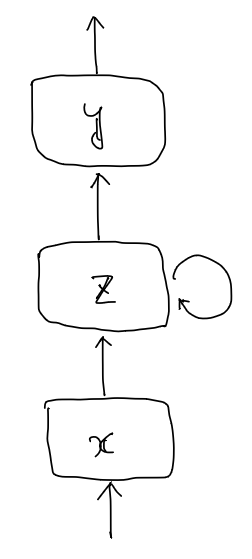
\includegraphics[width=1.8cm, height=4.0cm]{figure/rnn.png}
        \end{column}
        %%% text - right
        \begin{column}[T]{0.80\textwidth}
            再帰型ニューラルネットワーク(reccurent neural network : RNN)
            \begin{itemize}
                \item 内部に閉路を持つニューラルネットの総称.
                \item (理論上)過去の全ての入力から一つの出力への写像を表現する.
                \item 系列データに対応.
            \end{itemize}
        \end{column}
    \end{columns}
\end{frame}


\begin{frame}
    \frametitle{RNNの伝播計算}
    \begin{itemize}
        \item RNNを時間方向に展開し,自己ループのない通常の順伝播型ネットワークと同様に扱う.
        \item 時間方向に展開すると深いネットワークとなり,勾配消失・勾配爆発につながる.
        \item 結果として,RNNの出力に反映できるのは高々10時刻程度.
    \end{itemize}

    \begin{figure}
        \begin{center}
            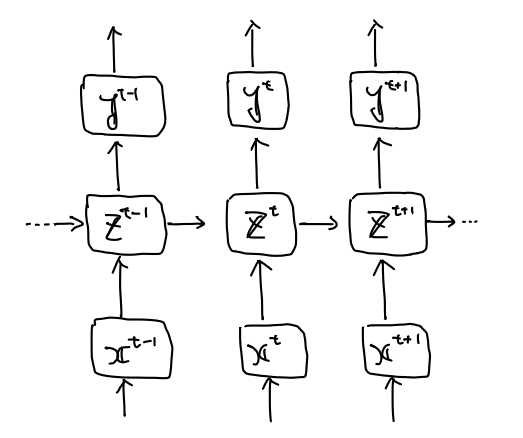
\includegraphics[width=6.0cm, height=4.6cm]{figure/rnn_exp.png}
        \end{center}
    \end{figure}
\end{frame}


\begin{frame}
    \frametitle{Long Short-Term Memory}
    長・短期記憶(long short-term memory : LSTM)
    \begin{itemize}
        \item RNNの勾配消失問題を解消して長期間の記憶の実現を目指す.
        \item RNNの中間層の各ユニットをメモリユニットに置き換えた構造.
    \end{itemize}

    \vspace{\baselineskip}

    勾配消失問題について
    \begin{itemize}
        \item 解析の詳細は省略.
        \item 解決策 : 勾配消失回避のために自己ループの重みを1とする.
    \end{itemize}

    入出力重み衝突について
    \begin{itemize}
        \item 入力を伝達させたい vs 入力を止めたい (出力も同様)
        \item この競合が学習が遅れる原因になってしまう.
        \item 解決策 : 入出力ゲートを導入.
    \end{itemize}
\end{frame}


\begin{frame}
    \frametitle{LSTM \small{メモリセル/入出力ゲート}}
    \begin{columns}
        %%% figure - left
        \begin{column}[T]{0.60\textwidth}
            \centering
            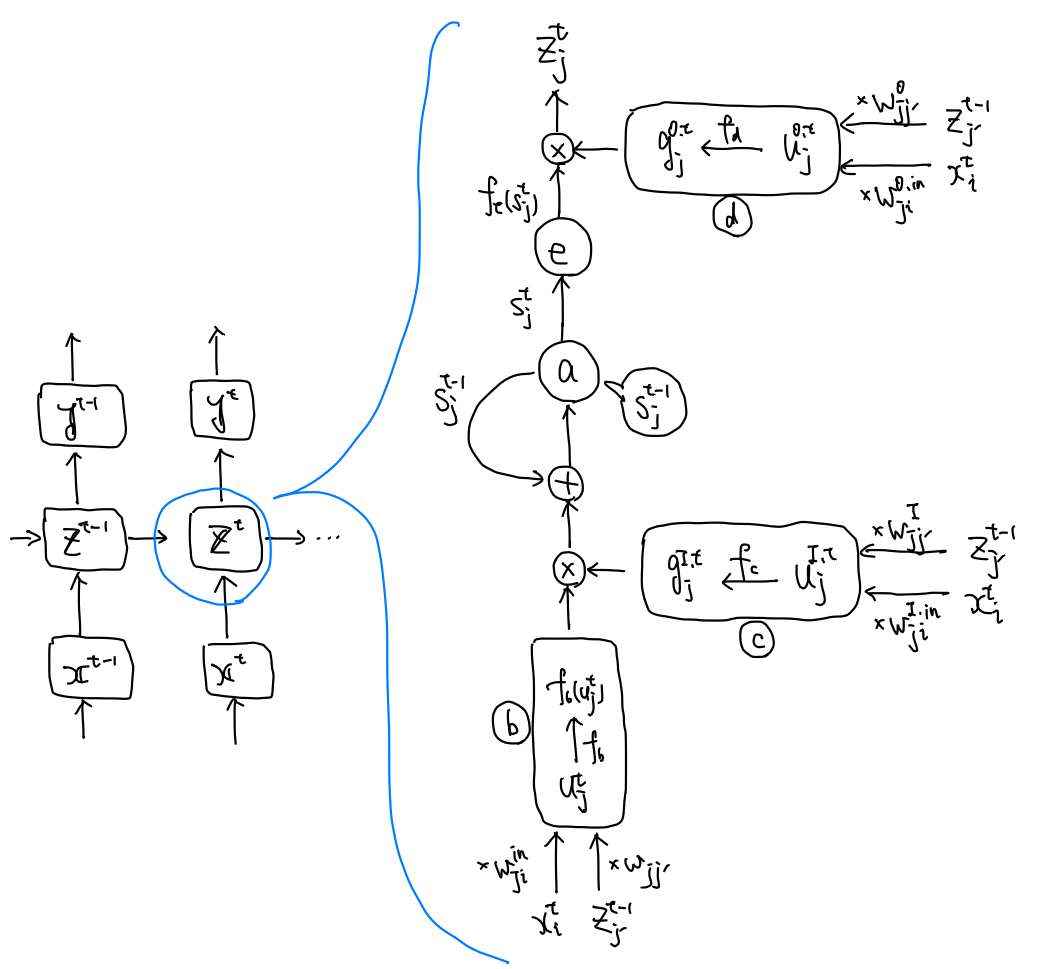
\includegraphics[width=7.2cm, height=7.2cm]{figure/lstm_original.png}
        \end{column}
        %%% text - right
        \begin{column}[T]{0.40\textwidth}
            \begin{itemize}
                \item 勾配消失問題の解決を目指した.
                \item メモリセル(a) : 一時刻前の記憶$\s{j}{t-1}$を保持.
                \item ユニット(e) : メモリセルの出力$\s{j}{t}$に活性化関数$f_e$を適用.
                \item 入力ゲート(c),出力ゲート(d) : 入出力を間引く.
                \item $f_c = f_d = \sigma$ : ゲート値$\g{j}{I,t}, \g{j}{O,t}$を$[0, 1]$に制限.
                {\footnotesize ($\sigma (x) \coloneqq (1 + \exp(x))^{-1}$)}
            \end{itemize}
        \end{column}
    \end{columns}
\end{frame}


\begin{frame}
    \frametitle{LSTM \small{メモリセル/入出力ゲート}}
    \begin{itemize}
        \item これが最初に提案された形(1997年).
        \item メモリセル(a)はCEC(Constant Error Carousel)とも呼ばれる.
    \end{itemize}

    \vspace{\baselineskip}

    LSTM(メモリセル/入出力ゲート)の問題点
    \begin{itemize}
        \item メモリセルは記憶を保持し続ける.
        \item 入力系列のパターンが大きく変動したときに,不要な過去の記憶が残ったままになる.
        \item 不要になった過去の記憶を自動的に忘れるような構造にする.
        \item 解決策 : 忘却ゲートの導入.
    \end{itemize}
\end{frame}


\begin{frame}
    \frametitle{LSTM \small{忘却ゲート}}
    \begin{columns}
        %%% figure - left
        \begin{column}[T]{0.60\textwidth}
            \centering
            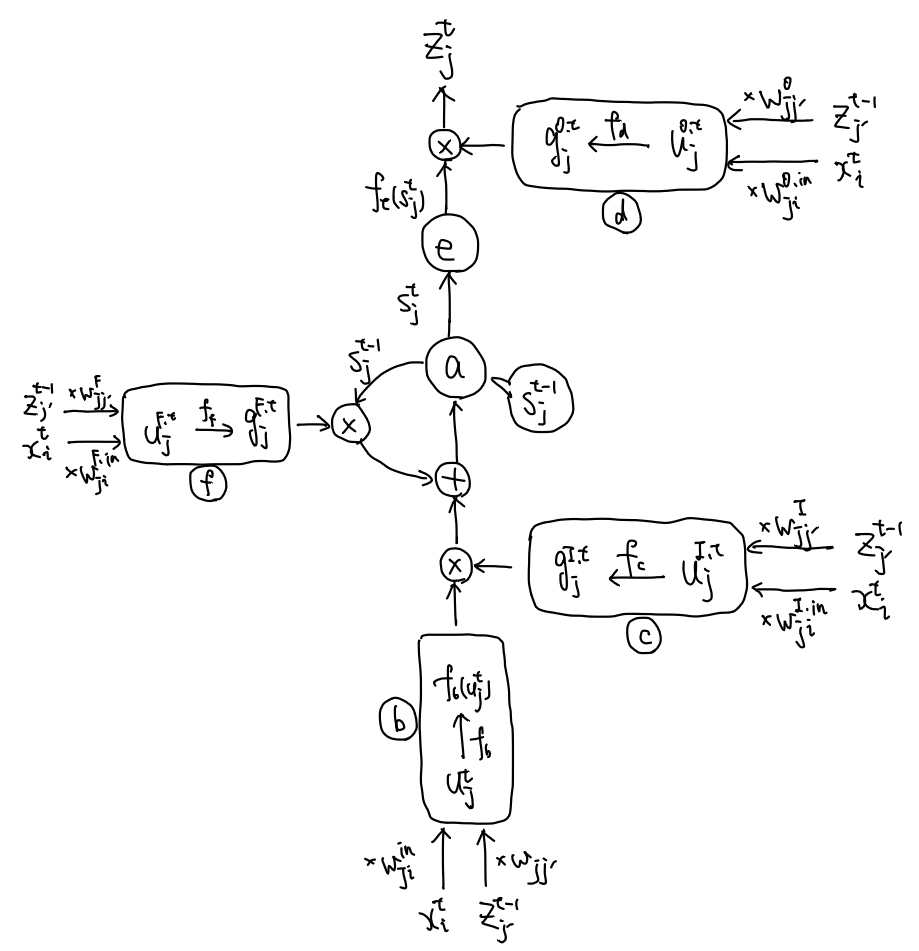
\includegraphics[width=7.2cm, height=7.2cm]{figure/lstm_fgate.png}
        \end{column}
        %%% text - right
        \begin{column}[T]{0.40\textwidth}
            \begin{itemize}
                \item 入力系列のパターンが大きく変動する場合に対応.
                \item 忘却ゲート(f) : メモリセルに記憶した情報$\s{j}{t-1}$を「忘れる」.
                \item 今までの記憶が不要になる(入力パターンが変動する)ときにメモリセルを初期化できる.
                \item $f_f = \sigma$ : ゲート値$\g{j}{F,t}$を$[0, 1]$に制限.
                {\footnotesize ($\sigma (x) \coloneqq (1 + \exp(x))^{-1}$)}
            \end{itemize}
        \end{column}
    \end{columns}
\end{frame}


\begin{frame}
    \frametitle{LSTM \small{忘却ゲート}}
    \begin{itemize}
        \item 忘却ゲートによって,不要になったメモリセルの内容を忘れることができるようになった.
    \end{itemize}

    \vspace{\baselineskip}

    LSTM(忘却ゲート)の問題点
    \begin{itemize}
        \item 各ゲートの役割は,
            \begin{itemize}
                \item 入力ゲート : メモリセルの内容を書き換えるか
                \item 忘却ゲート : メモリセルの内容を忘れるか(保持するか)
                \item 出力ゲート : メモリセルの内容を出力するか
            \end{itemize}
        であって,何れもメモリセルの制御が役割.
        \item ゲートは制御対象であるメモリセルの状態を直接参照できない.
        \item 解決策 : 覗き穴結合の導入.
    \end{itemize}
\end{frame}


\begin{frame}
    \frametitle{LSTM \small{覗き穴結合}}
    \begin{columns}
        %%% figure - left
        \begin{column}[T]{0.60\textwidth}
            \centering
            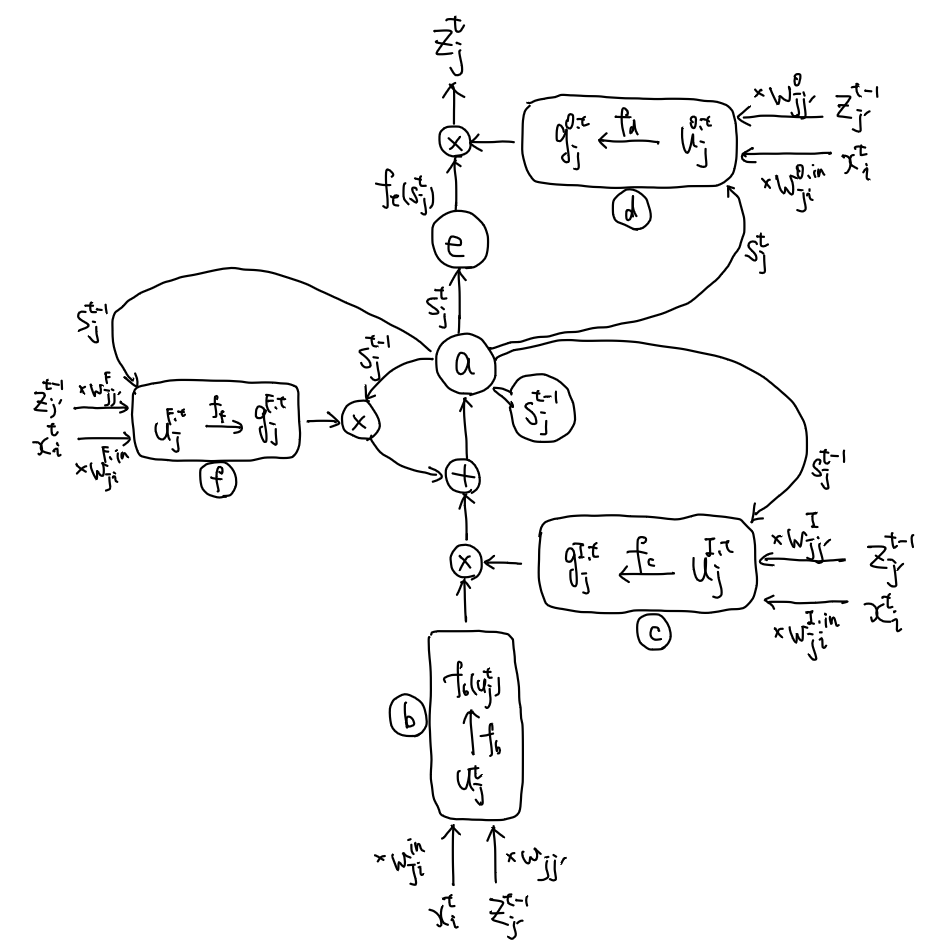
\includegraphics[width=7.2cm, height=7.2cm]{figure/lstm_peephole.png}
        \end{column}
        %%% text - right
        \begin{column}[T]{0.40\textwidth}
            \begin{itemize}
                \item ゲートの制御にメモリセルの内容を利用.
                \item これが教科書\cite{blue}に載っている形.
                \item 構造の詳細は異なることがある.
                    \begin{itemize}
                        \item 活性化関数$f_e$の省略
                        \item 覗き穴結合にも重み付け
                    \end{itemize}
            \end{itemize}
        \end{column}
    \end{columns}
\end{frame}


\begin{frame}
    \frametitle{LSTM概要図}
    \begin{columns}
        %%% figure - left
        \begin{column}[T]{0.5\textwidth}
            \centering
            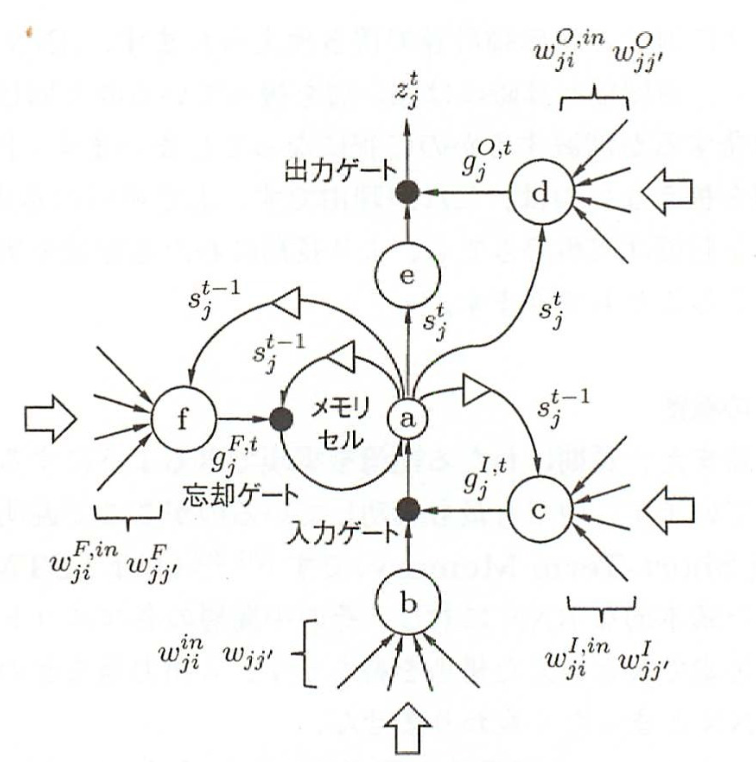
\includegraphics[scale=0.20]{figure/lstm.png}
        \end{column}
        %%% figure - right
        \begin{column}[T]{0.5\textwidth}
            \centering
            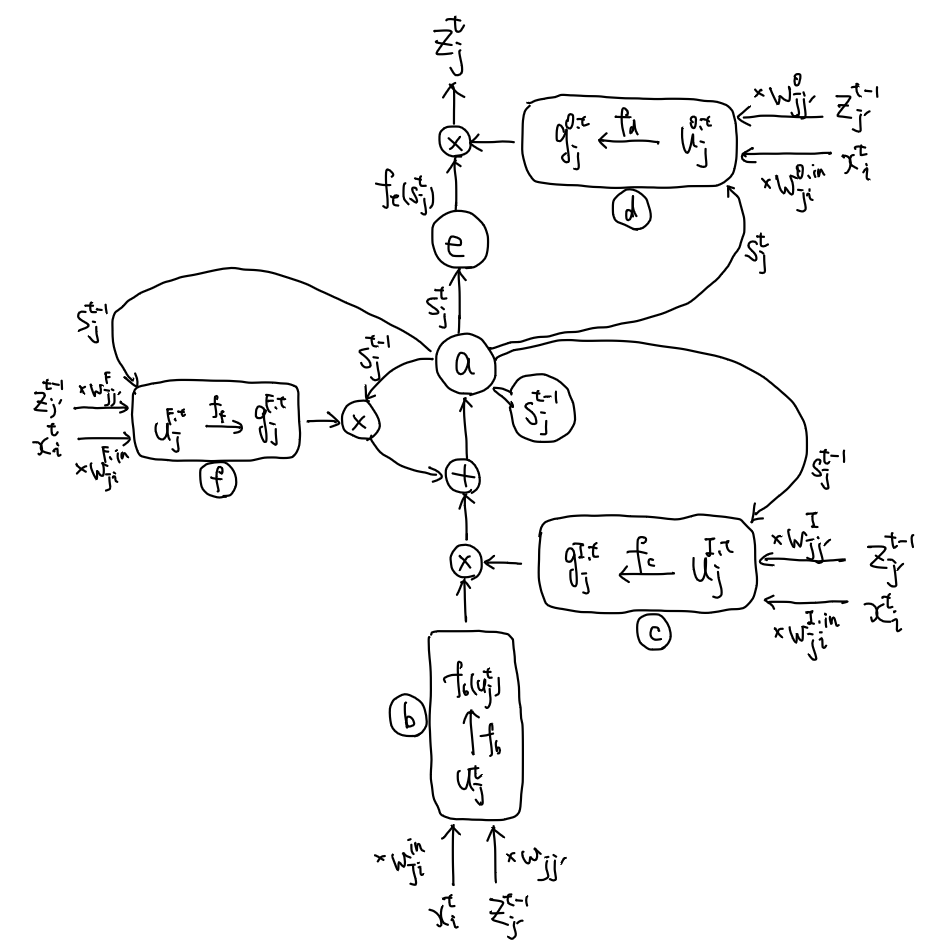
\includegraphics[width=5.8cm, height=5.8cm]{figure/lstm_peephole.png}
        \end{column}
    \end{columns}
\end{frame}


\begin{frame}
    \frametitle{順伝播計算}
    順伝播計算は次のようになる.
    \begin{align*}
        &\z{j}{t} = \g{j}{O,t} f(\s{j}{t}) \\
        &\g{j}{O,t} = f_d(\u{j}{O,t})
                   = f_d \left(\sum_{i} \w{ji}{O,in} \x{i}{t} + \sum_{j'} \w{jj'}{O} \z{j'}{t-1} + \s{j}{t} \right) \\
        &\s{j}{t} = \g{j}{F,t} \s{j}{t-1} + \g{j}{I,t} f_b(\u{j}{t}) \\
        &\g{j}{F,t} = f_f(\u{j}{F,t})
                    = f_f \left( \sum_{i} \w{ji}{F,in} \x{i}{t} + \sum_{j'} \w{jj'}{F} \z{j'}{t-1} + \s{j}{t-1} \right) \\
        &\g{j}{I,t} = f_c(\u{j}{I,t})
                    = f_c \left( \sum_{i} \w{ji}{I,in} \x{i}{t} + \sum_{j'} \w{jj'}{I} \z{j'}{t-1} + \s{j}{t-1} \right) \\
        &\u{j}{t} = \sum_{i} \w{ji}{in} \x{i}{t} + \sum_{j'} \w{jj'}{} \z{j'}{t-1}
    \end{align*}
    (逆伝播は省略. 教科書\cite{blue}を参照.)
\end{frame}


\end{document}
